\chapter{Geometry and basic facts}

\section{Platonic and Archimedean solids}

Platonic solids are regular \textbf{convex} polyhedra. Regular polyhedron is a polyhedron whose all faces are congruent to a single regular polygon i.e. a polygon with all sides of equal length. There are exactly five Platonic solids: tetrahedron, cube, octahedron, dodecahedron and icosahedron.

Note that convexity is an important property for us, since it ensures, that we can always obtain a 3-vertex connected planar graph. This fact is also known as Steinitz’ theorem for polyhedra \cite{kendall24}.

The Archimedean solids can then be obtained by performing one of the following non-disjoint operations on Platonic solids:

\begin{description}
    \item[Truncation] Removes corners of the polyhedron by making a cut perpendicular to a line connecting the vertex of the corresponding corner with the centroid of the polyhedron.
    \item[Rectification] Special case of truncation where the truncating cuts are done in such way, that they go through midpoints of the edges connecting the vertices. 
    \begin{figure}[H]
        \centering
        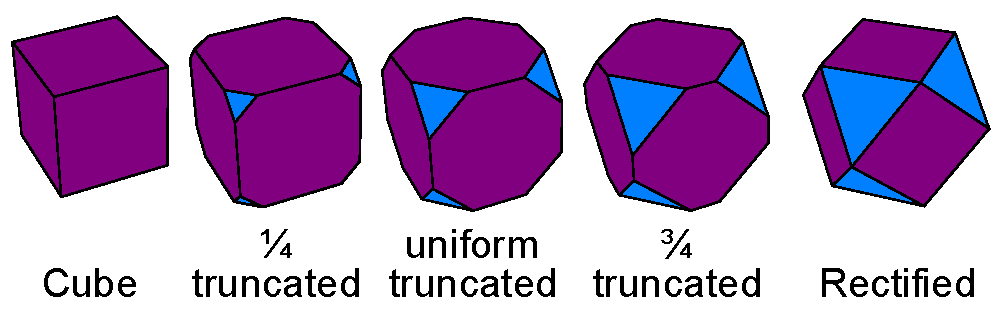
\includegraphics[width=1\textwidth]{../Resources/Figs/truncation.pdf}
        \caption{Trunctation and rectification operations visualised \cite{wikimedia-cube-truncation}}
        \label{fig:truncation}
    \end{figure}
    \item[Expansion/Cantellation] All the facets are pulled out away from the centroid of the polyhedron by the same distance without rescaling. The empty spaces are then filled with regular polygons in the following way: Edges that used to be identical in the original polyhedron are connected by adding a new a square. All the vertices that corresponded to a single vertex $v$ in the original polyhedron are connected by adding a $d$-gon where $d=deg(v)$.

    This operation can also be described as cantellation. The difference is in how we imagine the process that takes us to the resulting shape. From the viewpoint of cantellation, we first bevel (cut off) the edges and then apply truncation on what remained from the original vertices.
        \begin{figure}[H]
        \centering
        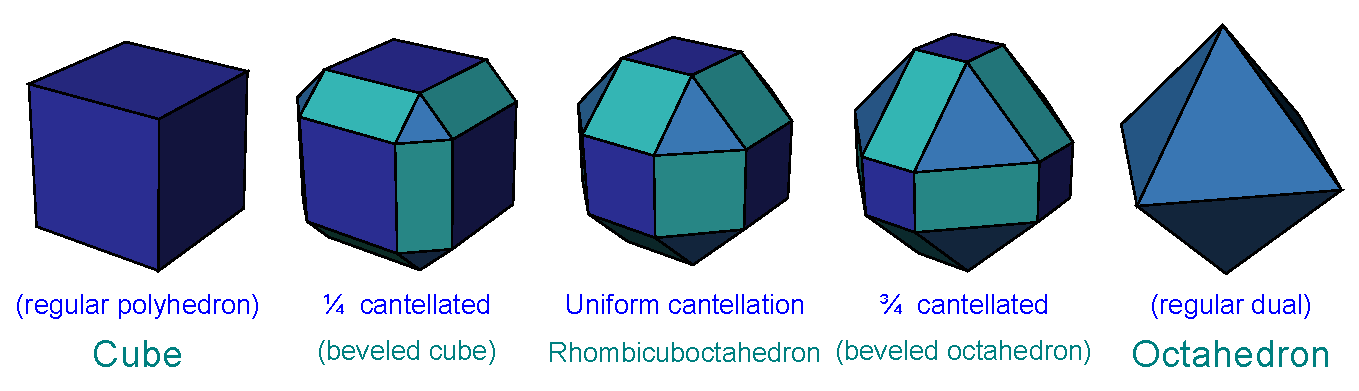
\includegraphics[width=1\textwidth]{../Resources/Figs/cantellation.pdf}
        \caption{Cantellation operation visualised \cite{wikimedia-cube-cantellation}}
        \label{fig:cantellation}
    \end{figure}
    \item[Snub] Is an application of expansion followed by splitting each new square in half in such a way, that we can twist the facets of the original Platonic solid.
\end{description}


\todo{TODO: Add visualisation of snub operation}

\section{Basic definitions and assumptions}

Here we state mathematical definitions, that should not be surprising in any way i.e. can be considered standard. Also, we state any assumptions we will make, which will then hold for the rest of this thesis.

\begin{definition}
    An \textit{undirected graph} $G$ is an ordered pair $G=(V,E)$ where $V$ is a set of vertices of the graph and $E \subseteq \binom{V}{2}$ is the set of its edges. 
\end{definition}

Since we are interested in Platonic and Archimedean solids, whose graphs are all planar, it is useful to define the notion of a \textit{plane graph}. This notion will correspond to a drawing of a particular graph onto a plane with one special property: the edges as they are drawn do not cross.

\begin{definition}
    Let $G=(V,E)$ be a graph. We call function $\varphi : V \cup E \rightarrow \mathbb{R}^2$ a \textit{drawing} of $G$ if it satisfies the following properties:
    \begin{enumerate}
    
        \item $\forall e=\{u,v\} \in E : \varphi(e)$ is a continuous line $\gamma$ whose endpoints are $\varphi(u)$ and $\varphi(v)$ such that $\gamma$ does not cross itself.
        
        \item (different vertices not drawn on same point) \\ $\forall u,v \in V : u \neq v \implies \varphi(u) \neq \varphi(v)$
        
        \item (edges not drawn onto non-endpoint vertices) \\ $\forall v \in V, \forall e \in E: v \notin e \implies \varphi(v) \notin \varphi(e)$
        
        \item (different edges can share only their common endpoints) \\ $\forall e \neq f \in E : x \in \varphi(e) \cap \varphi(f) \implies \exists v \in V: x = \varphi(v)$ and $v = e \cap f$
    \end{enumerate}
\end{definition}

A drawing of a graph might split the plane $\mathbb{R}^2$ into multiple separate segments. We will call these segments \textit{regions} of a drawing of graph $G$.

\begin{definition}
    A graph $G$ is \textit{planar} if there exists a drawing of $G$ into a plane.
\end{definition}

\begin{definition}
    A \textit{plane graph} $G' = (V,E,F)$ is a drawing of a planar graph $G=(V,E)$ into plane $\mathbb{R}^2$ where $F$ is the set of all regions of this drawing. We will also use the notation $V(G'), E(G'), F(G')$ to refer to sets $V,E,F$ respectively.
\end{definition}

In this thesis, we assume for any plane graph $G=(V,E,F)$ that the sets $V$, $E$ and $F$ are pairwise disjoint.


\section{Platonic and Archimedean graph properties}

Here we would like to list some properties, that the graphs corresponding to the solids described above. Let $G=(V,E,F)$ be a plane graph of a solid with faces $F$. In the following tables we use $v := |V|$ $e := |E|$, $f := |F|$ and $d$ is a number s.t. $\forall u \in V : \deg(u) = d$.

\vspace{5pt}
\todo[inline]{TODO: In tables below, include what n-gons the faces correspond to.}

\begin{table}[H]
\centering
\caption{Number of vertices, edges, faces and degree of each vertex of Platonic solids.}
\vspace{5pt}
\label{tab:platonic-basic-props}
\begin{tabular}{|l|c|c|c|c|}
\hline
Platonic & v & e & f & d \\
\hline\hline
cube & 8 & 12 & 6 & 3 \\
\hline
dodecahedron & 20 & 30 & 12 & 3 \\
\hline
icosahedron & 12 & 30 & 20 & 5 \\
\hline
octahedron & 6 & 12 & 8 & 4 \\
\hline
tetrahedron & 4 & 6 & 4 & 3 \\
\hline
\end{tabular}
\end{table}


\begin{table}[H]
    \centering
    \caption{Number of vertices, edges, faces and degree of each vertex of Archimedean solids.}
    \vspace{5pt}
    \label{tab:archimedean-basic-props}
    \begin{tabular}{|l|c|c|c|c|}
    \hline
    Archimedean & v & e & f & d \\
    \hline\hline
    cuboctahedron & 12 & 24 & 14 & 4 \\
    \hline
    icosidodecahedron & 30 & 60 & 32 & 4 \\
    \hline
    rhombicosidodecahedron & 60 & 120 & 62 & 4 \\
    \hline
    rhombicuboctahedron & 24 & 48 & 26 & 4 \\
    \hline
    snub cube & 24 & 60 & 38 & 5 \\
    \hline
    snub dodecahedron & 60 & 150 & 92 & 5 \\
    \hline
    truncated cube & 24 & 36 & 14 & 3 \\
    \hline
    truncated cuboctahedron & 48 & 72 & 26 & 3 \\
    \hline
    truncated dodecahedron & 60 & 90 & 32 & 3 \\
    \hline
    truncated icosahedron & 60 & 90 & 32 & 3 \\
    \hline
    truncated icosidodecahedron & 120 & 180 & 62 & 3 \\
    \hline
    truncated octahedron & 24 & 36 & 14 & 3 \\
    \hline
    truncated tetrahedron & 12 & 18 & 8 & 3 \\
    \hline
    \end{tabular}
\end{table}

